\section{Method}
\label{sec:method}
Figure~\ref{fig:method} summarizes the operator derived in this section as
an alternating cycle of task-direction distillation, latent optimization,
and frozen-prior regularization. The reference contrast supplies the task
direction, an RMS-normalized pseudo-target defines the latent objective,
and the reverse process advances the sample between interventions.

\subsection{Task and native reference conditioning}
\label{sec:conditioning}
Let $r$ denote the reference image and $c$ the full target instruction,
including the requested subject and transfer instruction. We consider two
objectives. \emph{Semantic style editing} seeks the requested subject in the
reference medium with substantial reference-layout retention.
\emph{Global style transfer} seeks the medium in an independently composed
image. In both cases, the target text specifies the output subject, while the
reference supplies the medium and, to a task-dependent degree, layout.

The frozen transformer predicts a velocity at latent $z_\sigma$ and noise
level $\sigma$. We query its native conditioning interface twice:
\begin{equation}
\begin{aligned}
v_r&=v_\theta(z_\sigma,\sigma,c,r),\\
v_b&=v_\theta(z_\sigma,\sigma,c,\varnothing).
\end{aligned}
\label{eq:branches}
\end{equation}
In the Klein implementation, the frozen VAE encodes the reference into
auxiliary image tokens. The transformer receives these tokens together
with the current noisy-image tokens and target-text representation.
Image-position identifiers distinguish the reference tokens from the
output tokens. The reference-free branch omits the auxiliary image tokens.
Text, latent state, noise level, and output geometry are shared between
the two queries, so their difference measures the response to adding the
reference condition.

\begin{figure*}[t]
\centering
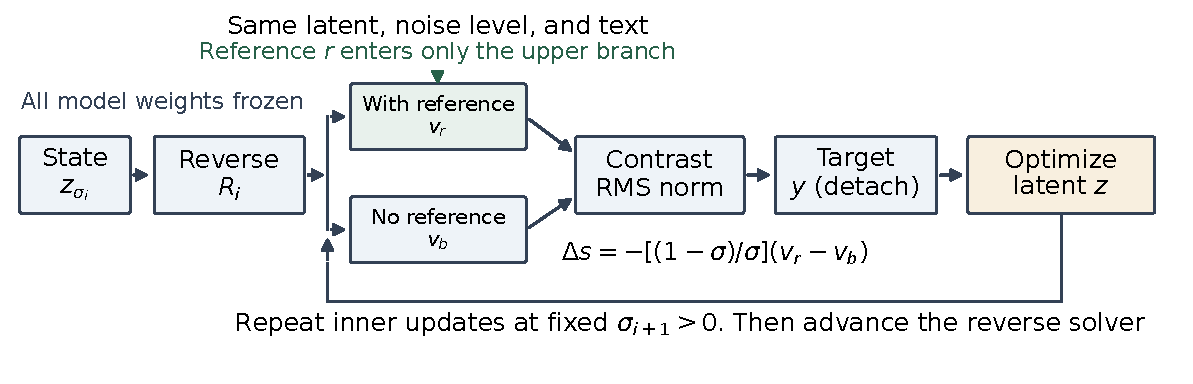
\includegraphics[width=\textwidth]{method.pdf}

\caption{TSD inference. The frozen reverse step reaches
$\sigma_{i+1}$, where paired reference-conditioned and reference-free
predictions define an RMS-normalized score direction. A detached target
then guides inner latent optimization at the reached noise level.
The cycle repeats with all network weights frozen.}
\label{fig:method}
\end{figure*}

\subsection{From velocity contrast to a score target}
\label{sec:target}
We express the native conditioning contrast in score space using the
rectified-flow interpolation
$z_\sigma=(1-\sigma)x_0+\sigma\epsilon$, with Gaussian $\epsilon$ and
velocity convention $v=\epsilon-x_0$. The clean estimate and score satisfy
\begin{align}
\hat x_0&=z_\sigma-\sigma v,\label{eq:clean}\\
s_\theta&=-\frac{z_\sigma+(1-\sigma)v_\theta}{\sigma}.
\label{eq:score}
\end{align}
Equation~\ref{eq:score} follows from the Gaussian-noise score identity with
the conditional-mean velocity. A learned field approximates that quantity
\citep{lipman2023flow,liu2023rectified}. The shared state cancels when the
two conditions in Eq.~\ref{eq:branches} are contrasted:
\begin{equation}
\Delta s_\sigma=s_r-s_b
=-\frac{1-\sigma}{\sigma}(v_r-v_b).
\label{eq:sign}
\end{equation}
The factor $-(1-\sigma)/\sigma$ fixes the orientation of the score
direction under this velocity convention. We clamp the denominator near
zero and apply optimization only at positive noise levels.

RMS normalization makes the target offset insensitive to most changes in
field magnitude across noise levels. For a positive multiplier $a$ and
normalization floor $\varepsilon_g$, define
\begin{equation}
g=a\Delta s_\sigma,\qquad
 d=\frac{g}{\max\!\left(\sqrt{N^{-1}\sum_{j=1}^N g_j^2},\varepsilon_g\right)},
\label{eq:normalization}
\end{equation}
where $N$ counts latent elements per sample. Away from the numerical
floor, the positive multiplier $a$ cancels under normalization. The
resulting direction has unit RMS, giving the target offset a consistent
scale across noise levels.

\subsection{RMS-normalized pseudo-target distillation}
\label{sec:optimization}
The pseudo-target supplies a first-order optimization signal without
backpropagating through the frozen transformer. With $\sg$ denoting
stop-gradient, each inner iteration forms
\begin{align}
\hat x_0(z)&=z-\sigma\sg(v_b),\\
y&=\sg\!\left(\hat x_0(z)+\eta d\right),\\
L_{\rm p}&=\frac{1}{2N}\sum_{j=1}^N(\hat x_{0,j}(z)-y_j)^2,
\label{eq:pseudoloss}
\end{align}
where $\eta$ sets the normalized target offset. Both teacher predictions
used to construct $d$ are detached and recomputed at the current inner-loop
state. The target is rebuilt before each loss evaluation, then treated as a
constant during differentiation.

Detaching the velocity makes the clean-estimate Jacobian the identity in
this branch. Thus
\begin{equation}
\frac{\partial\hat x_0}{\partial z}=I,
\qquad \nabla_z L_{\rm p}=-\frac{\eta}{N}d.
\label{eq:gradient}
\end{equation}
The mean reduction contributes $1/N$. For SGD with learning rate $\ell$,
the displacement is $\ell\eta d/N$. We use AdamW, whose moment estimates
and numerical stabilization determine the displacement from this gradient.
Thus $\eta$ controls the target offset and $\ell$ controls the optimizer
step. The supplementary derivation gives both update expressions.

The evaluated TSD operator uses $L_{\rm p}$ as its latent objective.
We initialize AdamW with zero weight decay at each outer intervention and
retain its moments across the inner iterations at that node. Recomputing
the target after every update keeps the reference contrast evaluated at
the current state. No warm-start or output AdaIN transformation is used.

\paragraph{Why a directional target?}
The target uses the direction of the reference contrast rather than a loss
that forces the two predictions to agree. Minimizing
$\frac12\|\Delta s(z)\|^2$ would differentiate the contrast itself and
produce $J_{\Delta s}(z)^\top\Delta s(z)$. Our detached target instead gives
the first-order direction in Eq.~\ref{eq:gradient}, without differentiating
the teacher. Normalization keeps the target offset informative even when
the contrast magnitude changes along the trajectory. Rebuilding the target
after each update lets successive interventions follow the reference
response at the edited state.

\subsection{Reverse-process regularization and style locality}
\label{sec:schedule}
The reference contrast provides a task direction, while the reverse field
provides the generative dynamics. This separation is motivated by the
CFG-augmentation and distribution-matching components of decoupled DMD
\citep{liu2025decoupled}. Their roles occur in different optimization
problems: DMD updates generator weights using a learned estimate of the
student distribution, whereas TSD updates one latent inside an existing
multi-step sampler. We retain that sampler as the regularizing component
of the inference procedure. No learned student-distribution estimate is
needed to define or execute the TSD operator.

We implement reverse-process regularization by alternating reference-directed
latent optimization with the frozen model's text-conditioned reverse steps.
The reverse solver advances the state before a guidance intervention. Let
$\sigma_0>\cdots>\sigma_M=0$ be its actual noise nodes and $R_i$ its reverse
update. From $z_{\sigma_i}$, we first obtain
$z^{(0)}_{\sigma_{i+1}}=R_i(z_{\sigma_i})$. If the reached positive node
belongs to the intervention set $\mathcal G$, we apply $K_i$ latent
optimization steps there. At other nodes we retain the solver output.
Algorithm~\ref{alg:tsd} specifies this order. The final reverse step has no
subsequent inner optimization.

\begin{algorithm}[t]
\caption{TSD inference}
\label{alg:tsd}
\begin{algorithmic}[1]
\REQUIRE Frozen $v_\theta$, instruction $c$, reference $r$, solver nodes,
interventions $\mathcal G$, inner counts $K_i$, $\eta$, optimizer rate $\ell$
\STATE Initialize Gaussian latent $z_{\sigma_0}$
\FOR{$i=0,\ldots,M-1$}
\STATE $z\gets R_i(z_{\sigma_i})$ at $\sigma_{i+1}$
\IF{$\sigma_{i+1}\in\mathcal G$ and $\sigma_{i+1}>0$}
\STATE Initialize latent optimizer at $z$
\FOR{$k=1,\ldots,K_i$}
\STATE Evaluate detached $v_r,v_b$ at the same $(z,\sigma_{i+1},c)$
\STATE Construct $d$, $y$, and $L_{\rm p}$ using Eqs.~\ref{eq:normalization}--\ref{eq:pseudoloss}
\STATE Update only $z$ using $\nabla_z L_{\rm p}$
\ENDFOR
\ENDIF
\STATE $z_{\sigma_{i+1}}\gets z$
\ENDFOR
\STATE Decode $z_{\sigma_M}$
\end{algorithmic}
\end{algorithm}

\paragraph{Style locality and working points.}
The solver nodes determine where reverse sampling evaluates the model,
while $\mathcal G$, $K_i$, $\eta$, and $\ell$ determine the latent
interventions. We use their joint settings to obtain different degrees of
style strength and reference-layout retention. The retained configurations
use 25 reverse intervals with two inner updates and $\eta=.05$, or eight
intervals with five inner updates and $\eta=.12$. Both use learning rate
$.01$. Inner updates occur after eligible positive reverse nodes.
For controlled comparisons of discretization, we also insert shared
positive nodes and assign the same inner count at each node. This separates
solver resolution from intervention location and count.

\subsection{Relationship to CFG and computational cost}
\label{sec:controls}
Text guidance and reference guidance act on different conditions.
Let $v_u^\beta$ denote text CFG applied with image condition $u$, using
$v_{\rm uncond}+\beta(v_{\rm cond}-v_{\rm uncond})$ within that branch.
Direct reference guidance advances the reverse solver with
\begin{equation}
 v_{\rm refCFG}^{\beta}=v_b^{\beta}
       +\gamma(v_r^{\beta}-v_b^{\beta}).
\label{eq:referencecfg}
\end{equation}
Both image conditions use the same text scale $\beta$. In the retained TSD
settings, the reverse step uses the reference-free, text-guided velocity
$v_b^\beta$. Reference information enters through the inner score-contrast
target at fixed instruction $c$. The sampler text scale $\beta$, direct
reference scale $\gamma$, and score multiplier $a$ are recorded separately.

\paragraph{Computation.}
Each inner iteration evaluates the two frozen teacher branches and
backpropagates through the detached-target loss to the latent. The
transformer is evaluated under stop-gradient, so its activations need not
be retained for latent differentiation. With
$U=\sum_i K_i$ inner iterations, an uncached implementation adds $2U$
teacher evaluations to reverse sampling. Prediction sharing can reduce
this count. The cost analysis records model calls and latent backward calls. The final
latency and memory comparison will use common hardware with explicit
text-guidance and offload settings.
